\textbf{\large 11. FIR filters}
\\

\begin{align}
	H(\omega) &= \sum_{n=-\infty}^\infty h_n e^{-i \omega n} \\
	&= h_{-1} e^{i \omega} + h_0 e^{0} + h_1 e^{-i \omega} \\
	&= h_0 + h_1 \left( e^{i \omega} + e^{-i \omega} \right) & & \text{with}\ h_{-1} = h_1 \\
	&= h_0 + 2 h_1 \cos(\omega) \\
\end{align}


\textbf{a)} $\{h_{-1}, h_0, h_1\} = \left\{\frac{1}{3}, \frac{1}{3}, \frac{1}{3}\right\}$

\begin{equation*}
	H(\omega) = \frac{1}{3} + \frac{2}{3} \cos(\omega)
\end{equation*}

\textbf{b)} $\{h_{-1}, h_0, h_1\} = \left\{\frac{1}{4}, \frac{1}{2}, \frac{1}{4}\right\}$

\begin{equation*}
	H(\omega) = \frac{1}{2} + \frac{1}{2} \cos(\omega)
\end{equation*}

\textbf{c)} $\{h_{-1}, h_0, h_1\} = \left\{-\frac{1}{4}, \frac{1}{2}, -\frac{1}{4}\right\}$

\begin{equation*}
	H(\omega) = \frac{1}{2} - \frac{1}{2} \cos(\omega)
\end{equation*}

\vspace{1cm}
Since all filters are symmetric around the orgin, the angles are zero.

\begin{figure}[h]
	\centering
	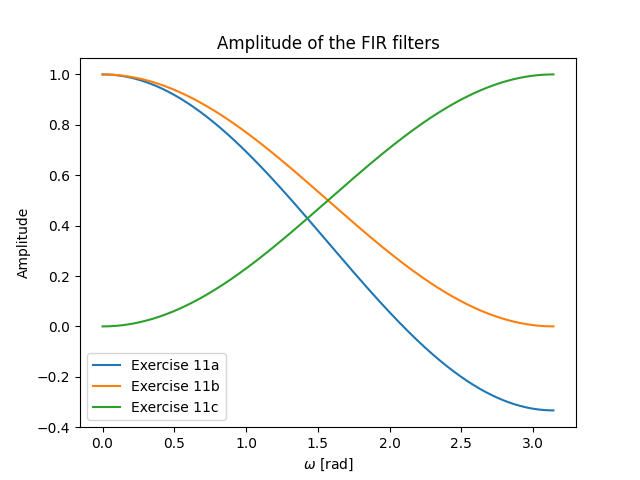
\includegraphics[width=12cm]{img/ex_11.png}
	\captionsetup{width=10cm}
	\caption{Amplitudes for the given FIR filters.}
\end{figure}


